\begin{figure}[h!]
    \centering
    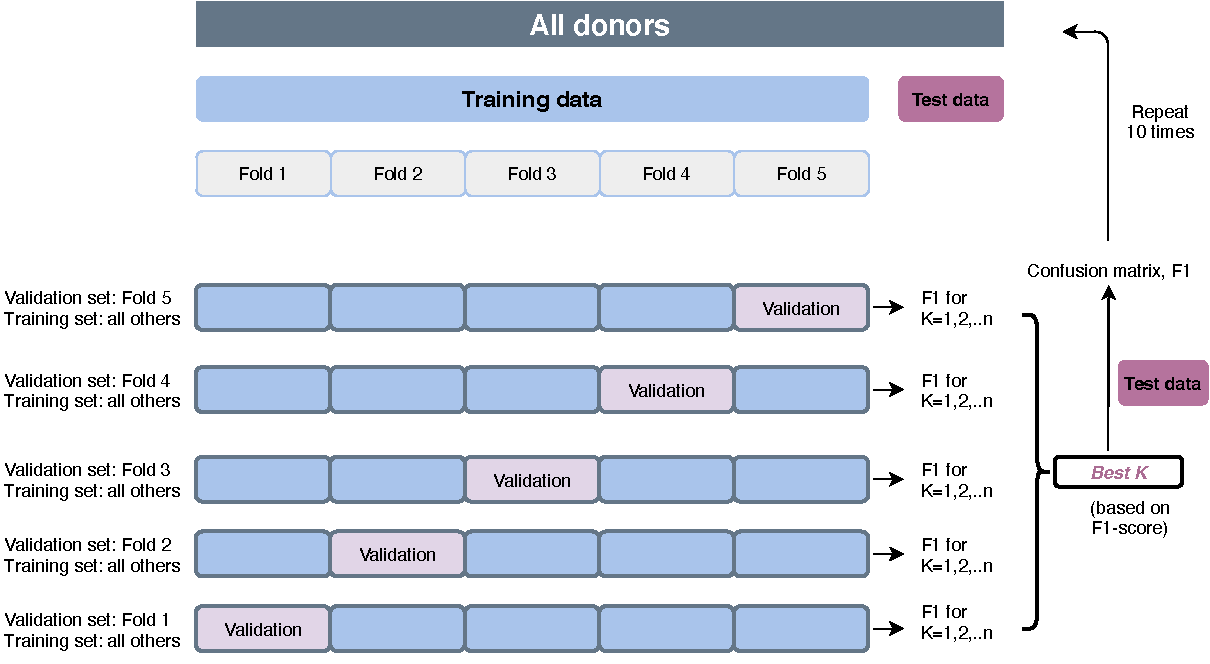
\includegraphics[scale=0.8]{graphics/ML_demo.pdf}
    \caption{\textbf{Illustration of machine learning cross validation workflow.} Data is split into a test set (1/10) and a training set (9/10). The training set is divided into 5 folds, each fold is sequentially used as a test set for model parameter selection. From 5 parameters set, I obtain the F1-score on the 1/10 test set to get the best parameter set. These parameters are then applied on the 1/10 test set for final evaluation, reported as a confusion matrix. The whole process is repeated 30 times to evaluate the possible range of the final confusion matrix.}
    \label{fig:ML_demo}
\end{figure}
